\documentclass[a4paper]{report}
\usepackage[italian,english]{babel}
\usepackage[utf8]{inputenc}
\usepackage{hyperref}
\usepackage{float}
\usepackage{graphicx}
\usepackage{gensymb}
\usepackage{graphicx}
\usepackage{float}
\graphicspath{.}

\setcounter{secnumdepth}{5} 	%per avere più livelli nei titoli
\setcounter{tocdepth}{5}		%per avere più livelli nell'indice

%----------------------------------------------------------------------------------------
%	TITLE PAGE
%----------------------------------------------------------------------------------------

\newcommand*{\titleGM}{\begingroup % Create the command for including the title page in the document
\hbox{ % Horizontal box
\hspace*{0.2\textwidth} % Whitespace to the left of the title page
\rule{1pt}{\textheight} % Vertical line
\hspace*{0.05\textwidth} % Whitespace between the vertical line and title page text
\parbox[b]{0.75\textwidth}{ % Paragraph box which restricts text to less than the width of the page

{\noindent\Huge\bfseries Tarrasque Engine 2.0}\\[2\baselineskip] % Title
{\large \textit{\\}}\\[4\baselineskip] % Tagline or further description
{\Large \textsc{Farine Antoine\\Storni Niko\\Ribeiro da Costa Nuno Miguel\\}} % Author name

\vspace{0.5\textheight} % Whitespace between the title block and the publisher
}}
\endgroup}


\begin{document}
\pagestyle{empty} % Removes page numbers
\titleGM
\tableofcontents
\pagenumbering{arabic}
\pagestyle{plain}
\setcounter{page}{1}

\chapter{Introduction}
Following the course of  ''Computer graphics'' we decided to enroll in the course of ''virtual reality''; this gave us the opportunity to further improve the graphic engine we developed during the previous semester. Additionally we also had the chance to get help from a new colleague that joined the group. In this course we learned the new features added in openGL from version 1.0 to version 4.4, moving from the fixed pipeline used in version 1.0 to the more programmable one that is used in 4.4. We also  learned techniques to efficiently use data in openGL and also multiple ways to render objects using stereoscopy to give a user the illusion of a real 3D virtual environment.\\
\chapter{From openGL 1.0 to 4.4}
This update was a two-step process, first, we updated to openGL 2.0 and from there we moved to openGL 4.4. The first step needed to accomplish that was using the new data structures in order to move data from the CPU to the GPU. To obtain these results we needed to use Vertex Buffer Objects. From that point we needed to add shaders to our graphic engine to successfully move to openGL 4.4.
\section{VBO}
To use vertex buffer objects successfully we needed to rework the way we loaded meshes from a file and how we rendered them. We started from the loading process, at first we simply loaded all the vertexes, normals and texture coordinates inside a TE\_Mesh object, but now it is not needed, we just need to load the vertexes, normals and texture coordinates on the GPU and then we store the vertex buffer objects ID returned to us by OpenGL in our Mesh object. We then implemented the rendering of the meshes using these new objects, to do that it was kind of how we rendered a texture in version 1.0: first we needed to enable a client state to tell OpenGL what we were binding, and then, once vertice, normals and texture coordinates were all bound we used a call to \emph{glDrawArrays} to draw the VBOs. This greatly improved the frame-rate in our graphic engine since most of the work is now done on to the GPU.

\section{Shaders}
After implementing the use of the more efficient data structures provided by OpenGL we needed to further improve our engine and this was done by implementing the use of shaders. We added a class to our engine that would handle the use of shaders, we reused the code provided by our teacher. The class TE\_Shaders lets us load, compile and build shader programs easily and then set the attributes and uniform variables.

In our engine we use a total of 3 shader programs: the first one is a \emph{per pixel shader} that renders our scene by computing the Blinn-Phong function for every fragment of the scene; the second one is a \emph{passthrough shader} used to render the framebuffer objects to the back-buffer; the last one is just a simple shader program used to render the skybox.

In our version of TE\_Shader we added several fields to the class so to store the ID of the attributes and uniforms loaded from the shaders so that we could easily retrieve them when needed while rendering. This is helpful, for example, in classes such as TE\_Material or TE\_Light

By using shaders we were able to implement per pixel lighting; this gave us the chance to surpass the old limitation of 8 maximum light sources per scene. However, in order to do that we needed to implement a new way of rendering our scene since the old way of enabling all the lights and then rendering the scene would not work anymore. Therefore implemented multipass rendering. Multipass rendering means that we render the entire scene multiple times and every time we render it we use a different light source, we use additive blending to accumulate the values in the buffer.\\
\begin{figure}[H]
\centering
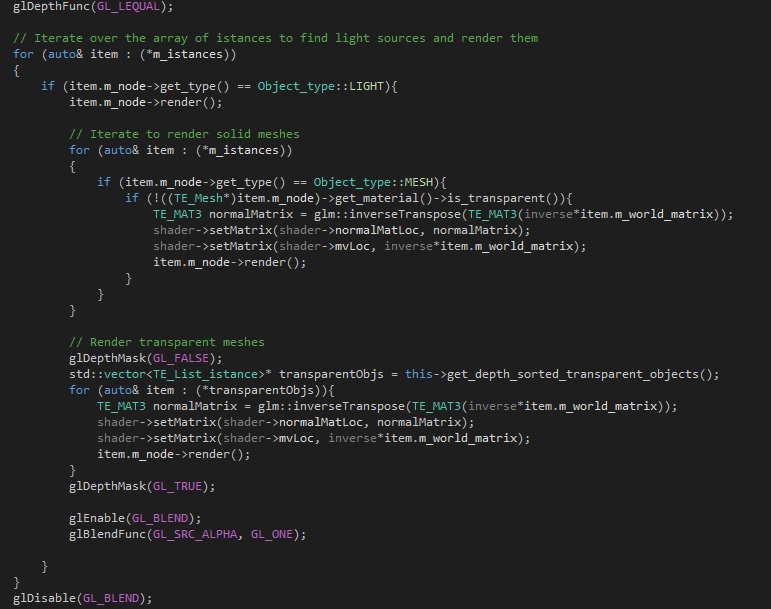
\includegraphics[scale=0.5]{multipass}
\caption{multipass rendering}
\end{figure}
The process of adding the use of shaders made us go through the rendering stages of the meshes again as we needed to tell the shader program what vectors, normals and texture coordinates to process during the rendering stages by setting their respective attributes and uniforms.

\chapter{Anaglyph rendering}

Once the rendering phase was completed and we were able to load a fully textured and lit scene, we needed to add a way to render anaglyphs with our engine. To do that we learned how to use frame-buffer objects as secondary buffers before rendering on the back-buffer. To use FBOs we added a class: TE\_Fbo, as we did with shaders. That helped us handle the creation, rendering and disposal of a frame-buffer. Again the code was provided by the teacher. 

To render anaglyphs we draw the scene twice: one time for the left eye and the second time for the right eye; to do that we use two frame-buffers, doing this will cut our frame-rate in half and that is why we needed to improve our data management so that we could provide 60 frames per second even when rendering the scene two times per display callback. In our engine we modified the display callback to reflect this change, we added a flag so that a client can easily switch rendering mode. In the stereoscopic mode we first render the scene from the left eye by applying an asymmetric frustum and moving the camera to the left, we do the same for the right frame-buffer and then we blend them using color-masks.\\
\\
In the engine the parameters required for setting the stereoscopic level such as the eye separation and the convergence plane are all customizable.
\chapter{Skybox}
To add a new layer of depth to our scene we then added a skybox; to render it correctly we created a new class GL\_SkyBox that would let us create and render it. To render the cube we created a special texture called cubemap, in OpenGL we used \emph{GL\_TEXTURE\_CUBE\_MAP}  instead of \emph{GL\_TEXTURE\_2D} this lets us generate a seamless texture in the shape of a cube. This process is similar to how we do in the TE\_Texture class as we use Freeimage to load the image into the engine and then we call \emph{glTexImage2D} to map the texture to the cubemap. \\
\begin{figure}[H]
\centering
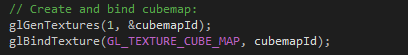
\includegraphics[scale=1]{cubemap}
\caption{Binding a cubemap}
\end{figure}
To render the skybox we built a new shader program, this one acts like the passthrough shader but here we need to flip the y coordinate of the texture since the skybox we downloaded is packed upside-down. It's also important that the skybox follows the camera rotations but not the translation, for this reason we pass the camera position matrix to the skybox and inside its render method we get the 3x3 portion that interests us and use it for the modelview matrix. We then call \emph{glDrawElements} to draw the faces of the cubemap.
\begin{figure}[H]
\centering
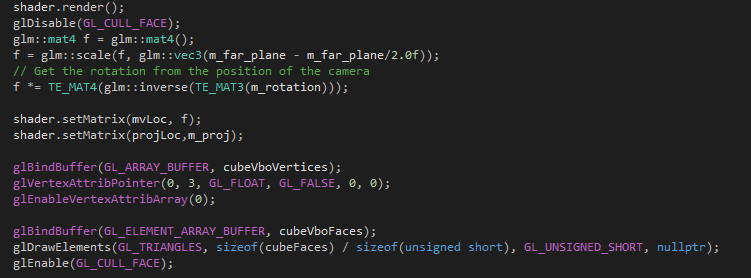
\includegraphics[scale=0.5]{skyboxRender}
\caption{Render function for skybox}
\end{figure}

\chapter{Arkanoid}
To test the new version of the engine, the game \emph{Arkanoid} was implemented using the 3D stereoscopic vision and the LeapMotion controller as an input source to move the bar.\\

\section{The game}
Arkanoid is an old video game where the player uses a base bar, that only moves on the x-axis, to bounce a constantly moving ball in order to destroy arrays of blocks standing still on top of the scene. The objective of the game is to get rid of all the blocks without letting the ball fall below the bar itself.\\
\begin{figure}[H]
\centering
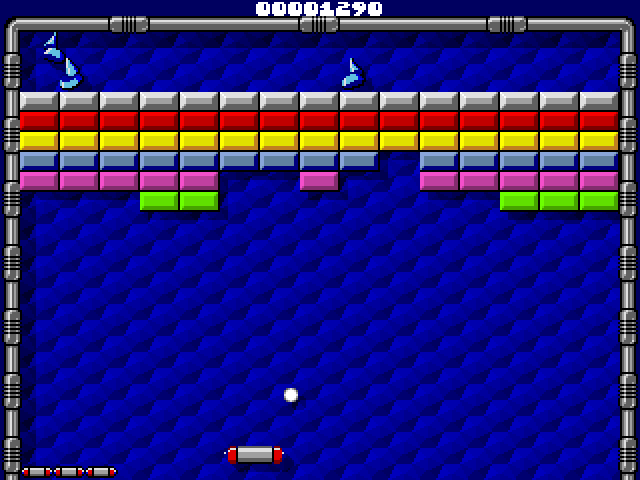
\includegraphics[scale=0.45]{Arkanoid}
\caption{Game example}
\end{figure}

The logic implemented in this game is pretty simple: the ball has a directional vector that increases the position of the ball on each frame. When the ball exceeds the left or right most edge, the ball direction vector is mirrored on the x-axis. Similarly for the top most edge, the vector is mirrored on the y-axis.\\
On the bottom edge, a supplementary check is performed to verify whether or not the ball has hit the bar. \\
If the bar is hit, the ball bounces off as if it was colliding with an edge; otherwise the ball is lost and a new one is spawned.

The bar implements a feature where if the ball hits it on the left/right most side, the resulting mirrored directional vector is slightly increased on the x-axis to add some sort of directional control for the player.\\
The top blocks are arranged in three rows and each time the ball enters the region of one of one row, each block belonging to the line is tested against the ball position; if the block happens to correspond to the position of the ball, then we consider it being hit and the function responsible for this check returns the following values:
\begin{itemize}
\item 1 if the block is hit from the top or the bottom
\item 2 if the block is hit from the left or the right side.
\item 0 if there is no actual collision
\end{itemize} 

Given the returned value we can calculate the proper direction the ball must take when bouncing off.

Once a block is hit, it's removed from the scene and the block is marked as removed. Once all the blocks are removed the game ends.\\
\begin{figure}[H]
\centering
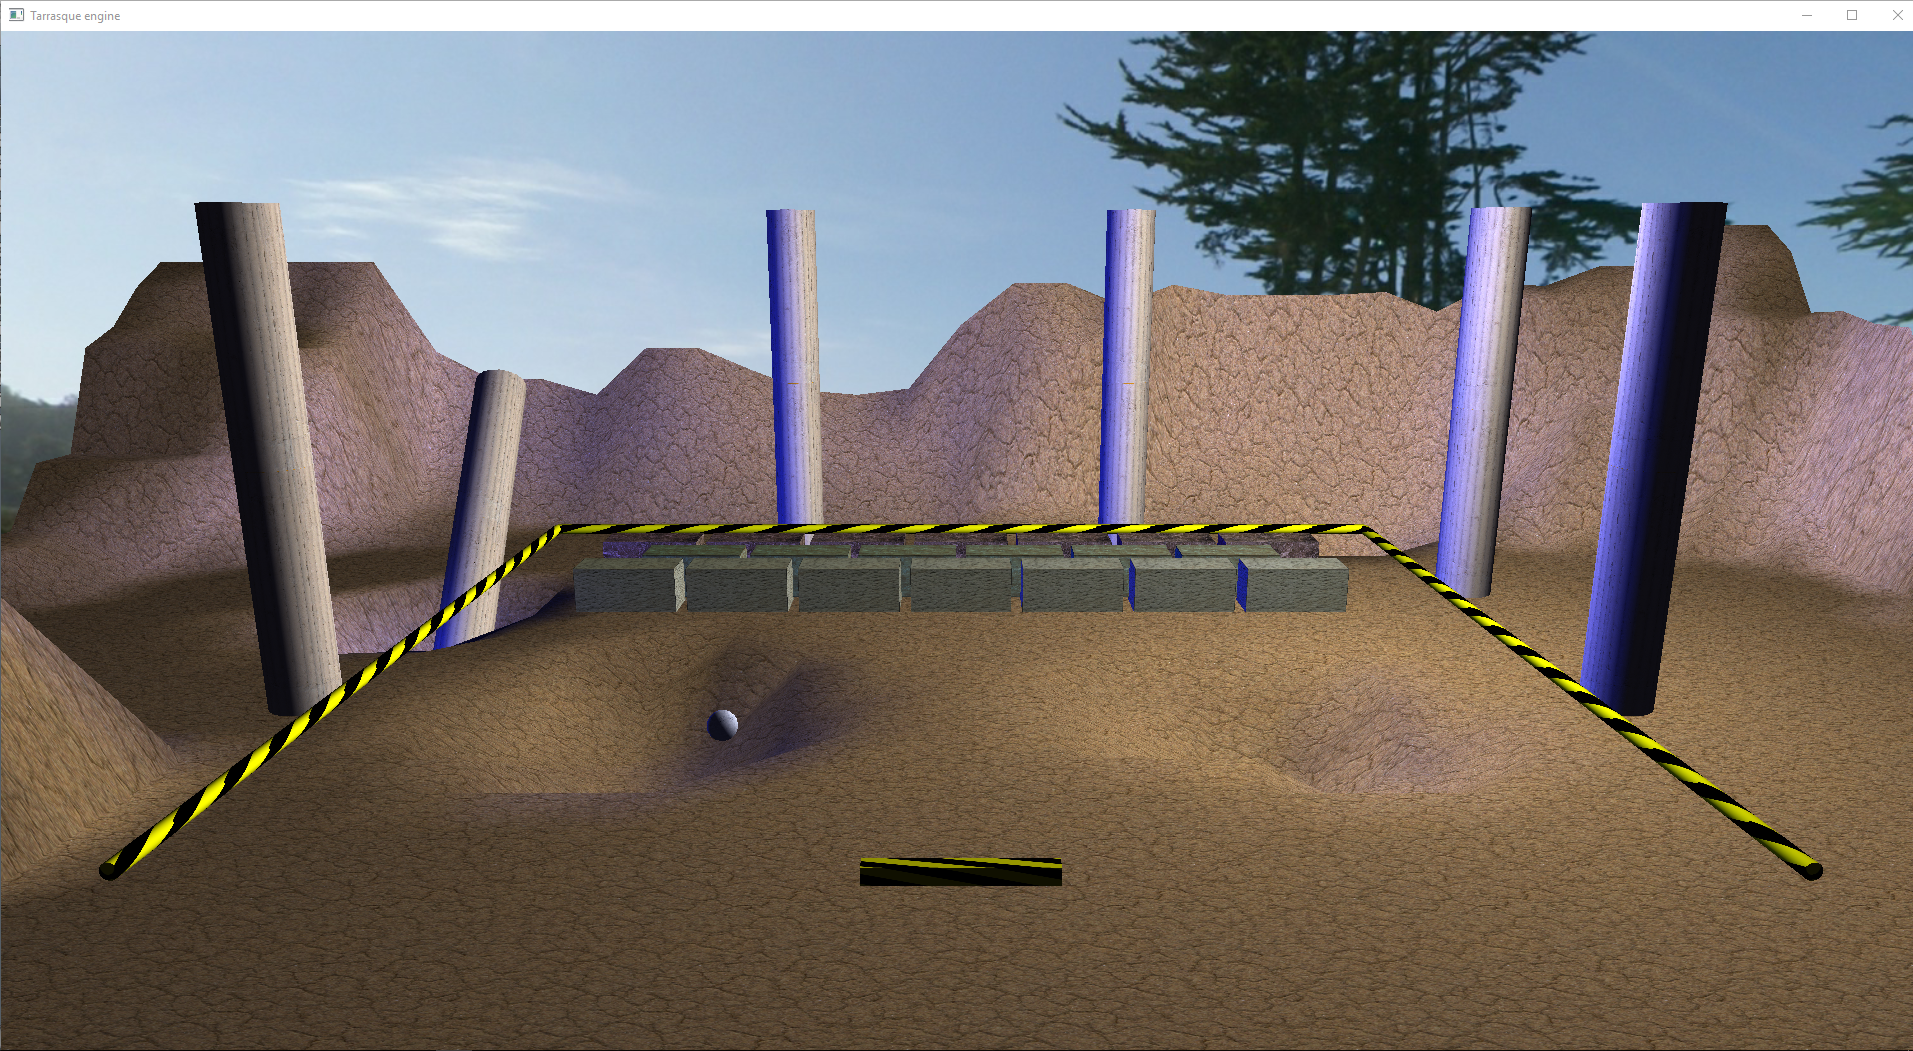
\includegraphics[scale=0.25]{Arkanoid3D}
\caption{Implemented version of the game}
\end{figure}

\section{Leap Motion}
The LeapMotion controller is the primary input source for the player to interact with the game. 

In order to control our application with the LeapMotion we had to download the SDK provided with the hardware. The SDK offers much more than we require; here are the steps we needed to take in order to integrate this controller with our game.

The LeapMotion has an object \emph{Controller} which connects to the physical controller and returns information regarding its field of view stored in a frame. The frame is a snap of a predefined area around the LeapMotion controller in which it is able to detect the presence of one or more hands (as well as all their properties).
\begin{figure}[H]
\centering
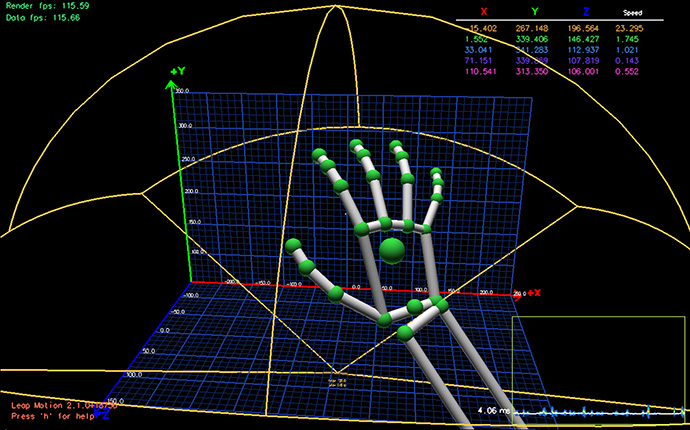
\includegraphics[scale=0.5]{Frame}
\caption{LeapMotion Frame}
\end{figure}
The controller has a listener which can be implemented by the developer to listen on the methods onCreate and onFrame. The first one is called when the LeapMotion controller is connected and the second one is called each time there is an update on the Frame. \\
In this second method, a reference to the hand position is updated to keep track of it. This same value is then used in the display callback to update the position of the bar so that the hand and the bar are always aligned.\\


\end{document}